We aim in this chapter to answer the question of why is statistical mechanics suitable for studying of Economic systems. The answer in essence is that the techniques of physics allow for one to find the minimum energy configuration (or at least very good approximations) for rather complicated settings, which is precisely what economics could mostly benefit of. 

To the reader familiar with statistical mechanics, we draw attention to the fact that we present here the canonical ensemble not as a derivation from thermodynamics, but as an inference using information theory. Instead of assuming a system connected to a heat bath at a fixed temperature and employing the first postulate of statistical physics, we follow the work of Jaynes \cite{Jaynes57} and show that the Gibbs distribution is the solution for an inference problem with limited information.

\section{Statistical Mechanics as an inference problem}

Suppose we have an interacting system composed of $N$ particles, each with its own state $x_i$, which can be its position, velocity, orientation, decision of whether to buy a Mac or a PC, etc. The whole system can be fully characterized by the configuration vector $x = (x_1, \ldots, x_N)$ and we assume all the information we have about this system is the expected value of an energy function $H(x)$. We would like to know what is the probability of this system being at a configuration $x$, or what is the expected value of another quantity $G(x)$. These questions are inference problems, and they can be solved in a principled way through information theory.

As proposed by Shannon \cite{shannon1948}, when faced with a choice of several probability functions, one should always opt for that which makes the least assumptions possible given its constraints. This amount to finding the probability distribution $p(x)$ that maximizes the \textbf{Shannon entropy}

%TODO: show the shannon entropy in an Appendix maybe?
\begin{equation}
    S[p] = - \int dx P(x) \log P(x)
\end{equation}
subject to the constraints imposed by observation. In our case, the constraint is that the energy function $H(x)$ has an average value $\langle H(x) \rangle = \int dx \, P(x) H(x) = E$ and we also have to impose the constraint that $P(x)$ is a probability distribution and therefore must be normalized, i.e., $\int dx \, P(x) = 1$. This means to find $P(x)$ for our system, we must find $P(x)$ that maximizes the Lagrangian

\begin{equation}
\mathcal{L}(P) =  - \int dx P(x) \log P(x) + \alpha \left(\int dx \, P(x) - 1\right) + \beta \left( \int dx \, P(x) H(x) - E \right),
\end{equation}
where $\alpha$ and $\beta$ are the Lagrange multipliers of this maximization problem. 

We assume that at the maximum $P^\ast$ a small perturbation $P(x) + \delta P(x)$ doesn't alter the Shannon entropy. If we assume that all $\delta P(x)$ are independent (i.e., $\delta P(x)$ and $\delta P(x')$ are not correlated, then for every $x$ this becomes a regular maximization problem. For every $x$, we must solve that $\partial \mathcal{L}(P) \partial P(x)$ is equal to zero, that is:

\begin{equation}
\frac{\partial}{\partial P(x)}\left\{ -P(x) \log P(x) + \alpha \left(P(x) - 1\right) + \beta \left(P(x) H(x) - E\right) \right\} = 0, \quad \forall x  
\end{equation}

Solving this equation we have that for every value of $x$

\begin{align}
    & -\log P(x) - 1 + \alpha + \beta H(x) = 0 \Rightarrow \\
    & \Rightarrow  P(x) = e^{1 - \alpha - \beta H(x)}
\end{align}

The Lagrange multipliers must be set so that the constraints are satisfied. For $\alpha$ we have that $e^{1 - \alpha}$ must normalize the probability distribution, i.e.

\begin{align}
   &  \int dx e^{1 - \alpha - \beta H(x)} = 1 \Rightarrow \\
    & e^{-1 + \alpha} = \int dx e^{- \beta H(x)} = Z
\end{align}

This normalization term is the sum over all the configurations and is called the \textbf{partition function}. For $\beta$ we must have that 

\begin{equation}
    \int dx H(x) \frac{e^{-\beta H(x)}}{Z} = - \frac{\partial}{\partial \beta} \log Z = E
\end{equation}

That is, $\beta$ must be such that the average energy of the system is equal to the observed average $E$. However, suppose we haven't actually observed $E$, all we know is that it's fixed to some  value. Then, because $E$ is given by the above equation for which the only degree of freedom is a Lagrange multiplier, all the possible values it can take are given by varying $\beta$ from 0 to $\infty$. We have finally arrived at the maximum entropy distribution for our inference problem, which is the \textbf{Gibbs distribution}

\begin{equation}
\label{eq:gibbs}
    P (x | \beta) = \frac{1}{Z(\beta)} e^{-\beta H(x)},
\end{equation}

The extreme cases for $\beta$ give us an intuition on how the Gibbs distribution is distributed among all possible configurations. For $\beta = 0$, $P(x) = \frac{1}{Z}$, for all values of $x$. This means that in this limit all configurations are equally likely, regardless of their energy $H(x)$. In the opposite case, when $\beta \to \infty$, $Z$ becomes more and more concentrated around it's maximum point, where $E(x)$ is minimum, and eventually $P(x)$ collapses to a delta function around the minimum energy configuration, also known as \textbf{ground state} (it can also have an equal mass in several points in the case of multiple minima). Therefore, in the full spectrum, the Gibbs distribution begins completely uniform in the space of all configurations and slowly coalesces into the minimum energy values. If we assume $H(x)$ is bounded, then for every finite value of $\beta$, the system has a finite probability being in any configuration.

Likewise, the average value of another desired observable $G(x)$ is given by

\begin{equation}
g = \langle G(x) \rangle = \int dx \frac{1}{Z} e^{-\beta H(x)}
\end{equation}

Though we have called $H(x)$ the energy function for costumary reasons, this function is in principle arbitrary. However, for most systems of interest we can always decompose it as a sum of small scale interactions, that is, we can write

\begin{equation}
    H(x) = \sum_{a} H_a (x_a),
\end{equation}
where $a$ represent minimal cliques, usually pairwise, where we can reduce the interactions in the system to microscopic interactions. In this way, the behavior of macroscopic quantities such as the average energy or any other observable we are interested depends on the sum of a large amount of simple interactions. 


% TODO: phase transitions go here

We note that despite this being the standard theory for the canonical ensemble in statistical physics, so far we have not made any thermodynamical (or any other "physical") assumptions. We have been describing generic systems where we simply applied the tools of information theory for the inference of a random variable for which we have limited information. There's nothing that limits us to use the characterization of equation \eqref{eq:gibbs} only for gases in which the molecules interact according to the laws of physics. This is the fundamental reason why statistical mechanics is so successful at explaining such a varied wealth of phenomena: despite being developed first via physical laws, it is in fact universal.

The only real difference when dealing with a thermodynamical system is that when we plug the Gibbs equation back into the Shannon entropy we have

\begin{equation}
    S[P_G] = \log Z + \beta E
\end{equation}

Which is still general, but we can now use one of the Maxwell relations to give $\beta$ a physical interpretation:

\begin{equation}
   \frac{1}{T} = \frac{\partial S}{\partial E} = \beta
\end{equation}

Therefore in physical systems $\beta$ is identified as the inverse temperature and when $T \to infty$, the system assumes all possible configurations. Likewise, when $T = 0$, the system is frozen at the ground state. 


\subsection{A simple example}

We make explicit the general nature of the Gibbs distribution deduced in this section by a simple example\footnote{This example was taken from the course notes of Nestor Caticha.} of a random variable $x$ that can take three values: -1, 0 or 1. We know it's average is $\langle x \rangle = m$. What is the best inference we can make for it's probability distribution $P(x)$? The Gibbs distribution is

\begin{equation}
   P(x) = \frac{e^{-\lambda x}}{Z(\lambda)},
\end{equation}
where $Z(\lambda)$ is given by:

\begin{equation}
   Z(\lambda) = \sum_{x\in \{-1, 0, 1\} e^{-\lambda x}} =
   1 + 2\cosh \lambda
\end{equation}

And $\lambda$ is given by

\begin{equation}
   m = - \frac{\partial}{\partial \lambda} \log Z(\lambda) =  - \frac{2 \sinh \lambda}{1 + 2 \cosh \lambda}
\end{equation}

Writing $u = e^{-\lambda}$ and writing the hyperbolic functions as $2 \cosh \lambda = e^\lambda + e^{-\lambda}$ and $2 \sinh \lambda = e^\lambda - e^{-\lambda}$ we have

\begin{equation}
   \frac{u - u^{-1}}{1 + u + u^{-1}} = m \Rightarrow 
   m + (m+1)u + (m -1) u^{-1} = 0
\end{equation}

Multiplying both sides of the equation by $u$, we have the second order equation $(m - 1) u^2 + m u + (m + 1) = 0$, for which the (positive) solution is

\begin{equation}
   u = \frac{-m - \sqrt{m^2 - 4(m^2 - 1)}}{2 (m - 1)}
\end{equation}

\begin{figure}[!ht]
  \centering
  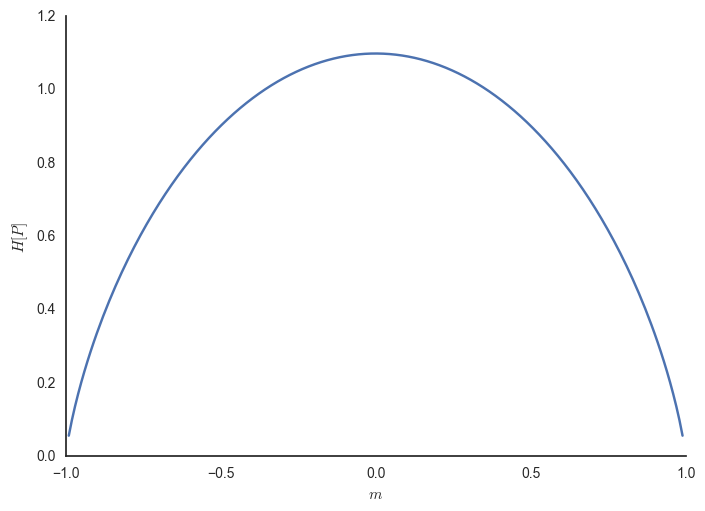
\includegraphics[width=0.4\textwidth]{figs_statmech/fig1a.png}
  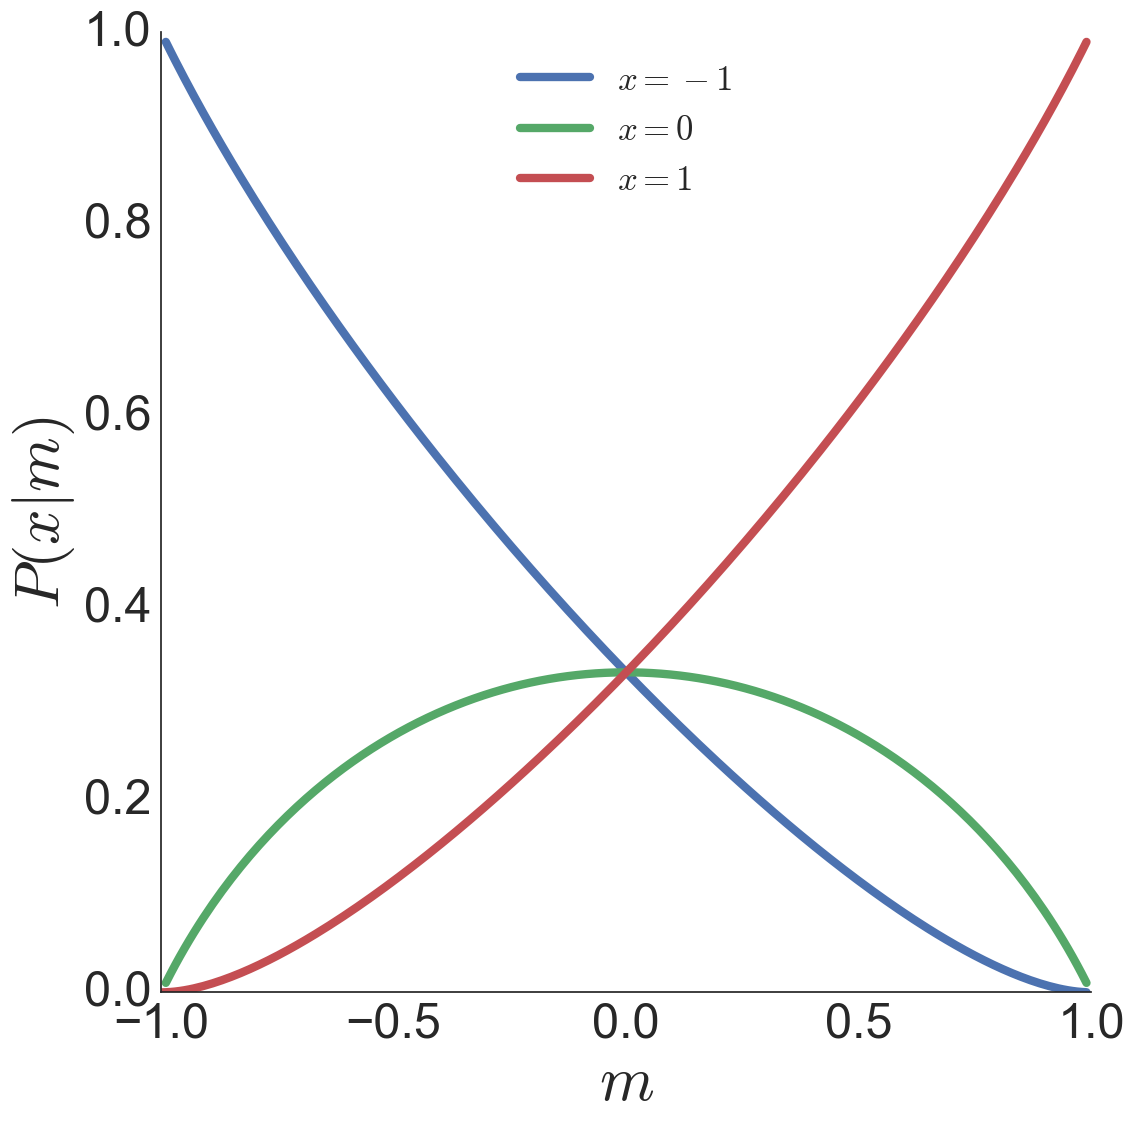
\includegraphics[width=0.4\textwidth]{figs_statmech/fig1b.png}
  \caption{\textbf{(Left)} Entropy $H[P]$ for the Gibbs distribution of a random variable $x$ that takes three values, -1, 0 and 1 as a function of its known average $\langle x \rangle = m$. \textbf{(Right)} Probability distribution $P_G(x|m)$ as a function of $m$ for each of the three values.}
  \label{fig:simple_example}
\end{figure}

And finally we find that $\lambda = -\log u$. We plot on Figure \ref{fig:simple_example} the entropy for the Gibbs distribution as a function of $\lambda$ and the probability $P(x|m)$ for the three values. We see that as expected entropy is maximal when the three states are equally likely, and when $m = \pm 1$ the variable is fully identified, so the entropy goes to zero.


\section{Optimization Problems}

The Gibbs distribution offers a natural way of solving maximization problems: given a system that we know has energy function $H(x)$, its ground state is simply the distribution of states $x$ at zero temperature, or at $\beta \to \infty$. Likewise, we can find any quantity of interest at maximum by computing $\langle G(x) \rangle$ in that limit. This is certainly not the only way one can find solutions to optimization problems, however, framing it as an statistical physics problem has a couple of benefits

% maximization problems as stat mech
% we can go beyond maximizations
% "dynamics" (ie, minority game)
% foley?
% phase transitions

\section{In Economics}

The suitability provided by statistical mechanics to economics problems has not gone unnoticed in Economics, even though it's usage is far from mainstream, starting from Santa Fe Institute's seminal work \textit{The economy as an evolving complex system} \cite{Anderson88, Arthur97}. In this section, we briefly describe some of the most relevant contributions from economics in the field. It's worth pointing out that, even when employed, rarely it is framed as a principled way of inference as we have presented in this chapter, instead statistical physics is usually arrived at through the addition of specially chosen stochastic terms that result in a Gibbs distribution.

In \cite{BrockDurlauf00} and \cite{BrockDurlauf01}, Brock and Durlauf 